\documentclass[twoside]{article}


\usepackage[sc]{mathpazo} % Use the Palatino font
\usepackage[T1]{fontenc} % Use 8-bit encoding that has 256 glyphs
\linespread{1.05} % Line spacing - Palatino needs more space between lines
\usepackage{microtype} % Slightly tweak font spacing for aesthetics

\usepackage[hmarginratio=1:1,top=32mm,columnsep=20pt]{geometry} % Document margins
\usepackage{multicol} % Used for the two-column layout of the document
\usepackage[hang, small,labelfont=bf,up,textfont=it,up]{caption} % Custom captions under/above floats in tables or figures
\usepackage{booktabs} % Horizontal rules in tables
\usepackage{float} % Required for tables and figures in the multi-column environment - they need to be placed in specific locations with the [H] (e.g. \begin{table}[H])
\usepackage{hyperref} % For hyperlinks in the PDF

\usepackage{lettrine} % The lettrine is the first enlarged letter at the beginning of the text
\usepackage{paralist} % Used for the compactitem environment which makes bullet points with less space between them

\usepackage{titlesec} % Allows customization of titles
\renewcommand\thesection{\Roman{section}} % Roman numerals for the sections
\renewcommand\thesubsection{\Roman{subsection}} % Roman numerals for subsections
\titleformat{\section}[block]{\large\scshape\centering}{\thesection.}{1em}{} % Change the look of the section titles
\titleformat{\subsection}[block]{\large}{\thesubsection.}{1em}{} % Change the look of the section titles

\usepackage{fancyhdr} % Headers and footers
\pagestyle{fancy} % All pages have headers and footers
\fancyhead{} % Blank out the default header
\fancyfoot{} % Blank out the default footer
\fancyhead[C]{USC EE511-PROJECT5} % Custom header text
\fancyfoot[RO,LE]{\thepage} % Custom footer text



\usepackage{multicol}
\usepackage{listings}
\usepackage{graphicx}
\usepackage{caption}
\usepackage{subcaption}
\usepackage{hyperref}
\usepackage{color}
\usepackage{float}
\usepackage{mathtools}
\usepackage{amssymb}
\usepackage{wrapfig}

\lstset{ %
language=Matlab,                % choose the language of the code
basicstyle=\footnotesize,       % the size of the fonts that are used for the code
numbers=left,                   % where to put the line-numbers
numberstyle=\footnotesize,      % the size of the fonts that are used for the line-numbers
stepnumber=1,                   % the step between two line-numbers. If it is 1 each line will be numbered
numbersep=5pt,                  % how far the line-numbers are from the code
backgroundcolor=\color{white},  % choose the background color. You must add \usepackage{color}
showspaces=false,               % show spaces adding particular underscores
showstringspaces=false,         % underline spaces within strings
showtabs=false,                 % show tabs within strings adding particular underscores
frame=single,           % adds a frame around the code
tabsize=2,          % sets default tabsize to 2 spaces
captionpos=b,           % sets the caption-position to bottom
breaklines=true,        % sets automatic line breaking
breakatwhitespace=false,    % sets if automatic breaks should only happen at whitespace
escapeinside={\%*}{*)}          % if you want to add a comment within your code
}

%----------------------------------------------------------------------------------------
%	TITLE SECTION
%----------------------------------------------------------------------------------------

\title{\vspace{-15mm}\fontsize{24pt}{10pt}\selectfont\textbf{Project \#5 - Markov Chains and discrete events}} % Article title

\author{
\large
\textsc{Li Yicheng}\thanks{\href{https://github.com/IAMLYCHEE/EE511-PROJ5}{github link: https://github.com/IAMLYCHEE/EE511-PROJ5} }\\[2mm] % Your name
\normalsize USCID:7827077047\\
\normalsize email: l.y.c.liyicheng@gmail.com \\ % Your institution
\normalsize USC Viterbi of Engineering
\vspace{-5mm}
}

\date{}

%----------------------------------------------------------------------------------------

\begin{document}

\maketitle % Insert title

\thispagestyle{fancy} % All pages have headers and footers
\section{Discrete Event Simulation}
\subsection{\normalsize{What this simulation can solve}}
The background problem mentioned in the project is to simulate how much time the server totally can have for break given the jobs come in a nonhomogeneous poisson distribution and the server's dealing time conforms the exponential distribution. This can also apply to how much time an agent in a telephone company can rest when the call coming in some distribution and the time spent on the phone call conforms to other distribution. The simulation is good for estimate a server's or an agent's workload and has profound application to adjust the allocation of jobs and the number of agents need for some particular task. 
\subsection{\normalsize{Simulation Routine}}
\begin{multicols}{2}
\subsubsection{Basic Framework}Generally, the server's next action is decided by whether there is a job waiting in his hand, if a job or jobs are still waiting, the simulation goes to a routine which concerns more about the dealing time and the next job come time. If there is no job waiting, the simulation goes to a routine which concerns more about the rest time and the next job come time. Therefore, every time the server start to serve, it detect the amount of jobs. We use variable nJobs to record the number of jobs waited to be served. And use Routine1 to mark server's reaction when nJobs is larger than 0 and use Routine2 to mark server's reaction when there is no job. Note, somewhere in the Routine1 all jobs may done, then, the server should go to routine2 and somewhere in routine2 when the jobs comes, the server go to routine1.\\
The following show the basic diagram: \\ 
\begin{figure}[H]
   \centering
   \includegraphics[width = 0.5\textwidth]{./data/outside.png}  
   \caption{basic framework}
\end{figure}
\subsubsection{Routine 1} denote `t' as the current time point, denote `tServe' as the time point indicating the starting time of service, denote tJob as the time point when the job comes. In routine 1 there are two cases: \\
\begin{figure}[H]
   \centering
   \includegraphics[width = 0.5\textwidth]{./data/routine1case1.png}  
   \caption{finish all jobs before the next job come}
\end{figure}
\begin{figure}[H]
   \centering
   \includegraphics[width = 0.5\textwidth]{./data/routine1case2.png}  
   \caption{haven't finish all jobs}
\end{figure}
\end{multicols}
\begin{multicols}{2}
In each case, the time shifts according to the time the server spent on the job, we use a loop to let the time shift and record how many jobs done. In the first case, all jobs are done before another jobs come, here we jump out of the loop and go to routine 2. In the second case, jobs still haven't done and another job already come. In this case, we set current time t back to the `next time when a job come'. And simulate how many more jobs come between the next server time between the `next job come time ' and 'the next server time'. And after this, set t to 'next server time' again which is just the routine 1 first case again. 
\subsubsection{Routine 2}
We use a loop to calculate how many breaks the server need to take before it can have a job to do, to simplify we just let time shift according to the break time until the service time is after the job come time. And when the condition meet, we set the current time to be the `job come time (tJob)' and use a loop to get how many more jobs done between the `tJob and tServe', after this, we meet the routin1 condition and we use routine 1 to keep going the simulation. 
\begin{figure}[H]
   \centering
   \includegraphics[width = 0.5\textwidth]{./data/routine2diagram.png}  
   \caption{how to break and start service}
\end{figure}
\end{multicols}
\subsection{\normalsize{code}}
With the above diagrams and figures, the following code can be more easy to understand, in the code, `generateBreakTime' is a function to generate break time, `nextJobComeTime' is a function to generate how much time it took for the next job to come, `generateExpDis(25)' is the function to generate how much time for the serve to deal with one job.
\noindent \textbf {Filename:generateTotalBreakTime.m} 
\begin{lstlisting}
function totalBreakTime = generateTotalBreakTime
%Li Yicheng 3/5
t = 0;
tServe = 0;
tJob = 0;
nJob = 0; %The number of jobs waiting to be served
totalBreakTime = 0;
stillJobs = false;
while t < 100
    if nJob == 0
        breakTime = generateBreakTime;
        tServe = tServe + breakTime;%service time after break
        tJob = tJob + nextJobComeTime2(t);%the time for the first job to come
        while tServe < tJob
            breakTime = generateBreakTime;%generate break time 
            tServe = tServe + breakTime;%next time to serve
        end
        %after this the time for serve is after the first job to be served
        totalBreakTime = totalBreakTime + tServe-t; %calculate the break time 
        t = tJob; % now set time to the first job come
        while t < tServe % calculate how many jobs come between first Job come time and serve time
            t = t + nextJobComeTime2(t); %next Job come time 
            nJob = nJob + 1; %Job amount plus one
        end
        %how many jobs waiting while the server is not coming back
        tJob = t; % now the t is the next Job come time
        t = tServe; % set time point to be the serve time start to serve
    else
        while tServe < tJob %how many jobs done before next job come
            tServe = tServe + generateExpDis(25); % time spent to next job
            nJob = nJob - 1; %job done
            if nJob == 0 % if all job finished
                stillJobs = false; %mark all job finised
                break;
            else
                stillJobs = true;
            end
        end
        if stillJobs == false % all job finish then set the current time 
            t = tServe ; 
        else % still some jobs
            t = tJob; %haven't finish when the next job come, set time to next job come
            while t < tServe %jobs come betwen this jobs come and next serve time
                t = t + nextJobComeTime2(t);
                nJob = nJob + 1;
            end
            tJob = t;
            t = tServe; %now continue to serve 
        end
    end
end

\end{lstlisting}
The above is the basic framework.\\
Following are the other codes for different time generating:\\
\noindent \textbf {generatelambda2.m}
\begin{lstlisting}
function lambda = generateLambda2(t)
to = t - floor(t/10) *10;
if to <= 5 
    lambda = 4 + 3 * to;
else
    lambda = -3 * to + 34;
end
\end{lstlisting}
\noindent \textbf {generatePoisSam.m}
\begin{lstlisting}
function i = generateaPoisSam(lambda)
%generate one poisson distribution
u = rand(1);
i = 0;
p = exp(-lambda);
F = p;
while u > F
    p = lambda * p / (i+1);
    F = F + p; %accumulate
    i = i+1;
end
\end{lstlisting}
\noindent \textbf {generateBreakTime.m}
\begin{lstlisting}
function t = generateBreakTime
t = rand(1,1) * 0.3;
\end{lstlisting}
\noindent \textbf {generateExpDis .m}
\begin{lstlisting}
function sample = generateExpDis(lambda)
%generateExpDis(lambda)
%generate a sample given exponential distribution
%input parameter: lambda
%using inverse transform sampling
p = rand(1,1)- 1.00e-10;
sample = log( 1- p) / (-lambda);
\end{lstlisting}

\section{Result}
To get the expectation, use the following script to repeat the experiment 200 times.\\
\begin{lstlisting}
%test 200 times 
breaktime = zeros(200,1);
for i = 1 : 200 
    breaktime(i) = generateTotalBreakTime;
end
histogram(breaktime,100);
title('breaktime distribution')
xlabel('total breaktime')
ylabel('appear times')
expectation = mean(breaktime);
\end{lstlisting}
\begin{multicols}{2}
\noindent \textbf {expectation = 25.0165} \\
This means the server averagely has 25 hours to rest in the first 100 hours. The next figure shows the distribution.
\begin{figure}[H]
    \centering
    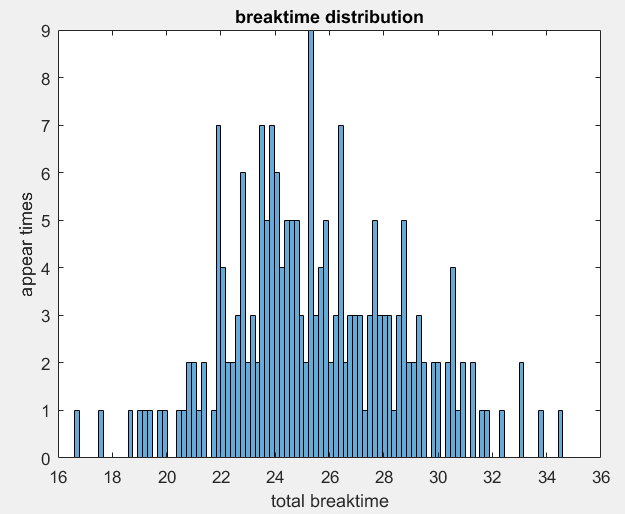
\includegraphics[width = 0.5\textwidth]{./data/breaktimeDistribution.png}  
    \caption{Distribution}
 \end{figure} 
\end{multicols}

\section{HOL-blocking switch performance}
\subsection{\normalsize{Background}}
In this task, we are to analyse a switch's performance which may have the head-of-line blocking problem. The following figure from Wikipedia describlem the situation well.
\begin{figure}[H]
   \centering
   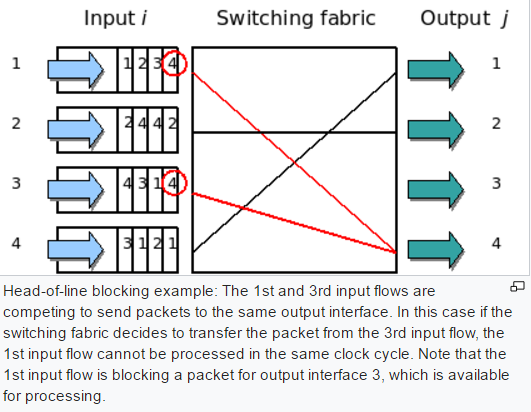
\includegraphics[width = 0.5\textwidth]{./data/HOLblocking.png}  
   \caption{https://en.wikipedia.org/wiki/Head-of-line\_blocking}
\end{figure}
\subsection{\normalsize{Implementation}}
\subsubsection{Algorithm}
It is easy to write the algorithm to simulate the situation. Use a variable to record how many packets in each input after some time, at each time slot, there are only four cases of the state: case1: input1 has packet(s) and input2 has no packet; case2: input1 has no packet, input2 has packet(s); case3: both input1 and input2 have packet(s); case4: neither has packet. For case1, the switch just let packet in input1 pass; for case2, the switch just let packet in input2 pass; for case3, there are two situation, first: both input have the same attempt to go to same output, leading to blocking situation; second: two inputs have different attempt and both of them passed the switch. The following diagram shows the flowchart:
\begin{figure}[H]
   \centering
   \includegraphics[width = 0.4\textwidth]{./data/diagram2.png}  
   \caption{Diagram for simulating the system}
\end{figure}
\subsubsection{Code}
\noindent \textbf {filename: numberInInput.m}
\begin{lstlisting}
function [nstate,efficiency_lyc,efficiency_tu] = numberInInput(p,r1,r2,tend)
%[nstate,efficiency_lyc,efficiency_tu] = numberInInput(p,r1,r2)
%output : 
%nstate : record how many packets in input1 and input2
%efficiency_lyc : records the efficiency according to my understanding of the
%efficiency
%efficiency_tu : records the efficiency based on the tutor's given definition
%input : p : the arriving probability
%r1 : the probability to target at output 1
%r2 : the probability to target at output 2 
%tend: continue entil tend
nstate = [p > rand(1) , p > rand(1)]; % nstate how many packet in each of the input
passed = 0;
maxpassed = 0;
% r1 = 0.5; r2 = 0.5;
attempt = [r1 > rand(1), r1> rand(1)];% nInput1 = nstate(1);
nextAttempt = [r1 > rand(1), r1> rand(1)];
% nInput2 = nstate(2);
priority = 1;
t = 1;
while t < tend
    if sum(nstate) > 0 
        if nstate(1) > 0 && nstate(2) == 0
            nstate(1) = nstate(1) - 1;
            passed = passed + 1;
            maxpassed = maxpassed + 1;
        else
            if nstate(1) == 0 && nstate(2) > 0
                nstate(2) = nstate(2) - 1;
                passed = passed + 1;
                maxpassed = maxpassed + 1;
            else % both have packet at the input
                if attempt(1) ~= attempt(2)
                    nstate = nstate - 1 ;
                    nextAttempt = [r1 > rand(1), r1 > rand(1)];
                    passed = passed + 2;
                    maxpassed = maxpassed + 2;
                else 
                    if priority == 1
                        nstate(1)= nstate(1) - 1;
                        priority = - priority;
                        nextAttempt = [r1 > rand(1),attempt(2)];
                    else
                        nstate(2) = nstate(2) - 1;
                        priority = -priority;
                        nextAttempt = [attempt(1), r1 > rand(1)];
                    end
                    passed = passed + 1;
                    maxpassed = maxpassed + 2;
                end
            end
        end
%     else
%         nextAttempt = [r1 > rand(1),r2 > rand(1)];
    end
    %new packet arrives
    nstate = nstate + [p>rand(1),p>rand(1)];
    attempt = nextAttempt;
    t = t + 1;
%     efficiency  = passed / t;
%     nstate
end
efficiency_lyc = passed /maxpassed ;
efficiency_tu = passed / (t*2);
\end{lstlisting}
Attention, here I output two kinds of efficiency, first is based on my understanding, because as far as I am concerned, the reason that cause the switch has low efficiency is that two packets have the same output to go, if an input has no packet, it is not to say the switch decreases its efficiency. So in my program, when a conflict occurs, that is the only place where I decrease my efficiency. But according to the material definition, every time slot the switch should pass a maximun of 2 packets, the efficiency is just the ratio of  number of passed packets and the 2 multiple the passed time slots. Anyway, I gave out two kind of efficiency calculation method. 

\subsection{\normalsize{Experiment \& Result:}}
\noindent \textbf {Plot the distribution and compute the mean of the number of packets in the buffer at input1 and input2 as a function of the arrival probability p.}\\
\begin{multicols*}{2}
\noindent \textbf \emph{parameter choosing:\\ tend = 200: run 200 time slot\\ In one given p, repeat the experiment 100 times to calculate the mean}\\
the following the script for the experiemnt:\\
\begin{lstlisting}
buffer = zeros(1,100);
k = 1;
for p = 0.1 : 0.05 : 1
    for i = 1 : 100
        [nstate,efficiency_lyc, efficiency_tu] = numberInInput(p,0.5,0.5,200);
        buffer(i) = sum(nstate);
        efficiency(i) = efficiency_tu;
    end
    recordNumber(k) = mean(buffer);
    recordEfficiency(k) = mean(efficiency);
    k = k+1;
end
plot(0.1:0.05:1,recordNumber);
title('packets in buffer given different p(200 time slots)');
xlabel('p');
ylabel('number of packet in buffer after 200 time slots');

plot(0.1:0.05:1,recordEfficiency);
title('efficiency given different p(200 time slots)');
xlabel('p');
ylabel('efficiency (\times 2 is the number of packet processed per time slot)');

\end{lstlisting}
\noindent \textbf {Result:}
\begin{figure}[H]
   \centering
   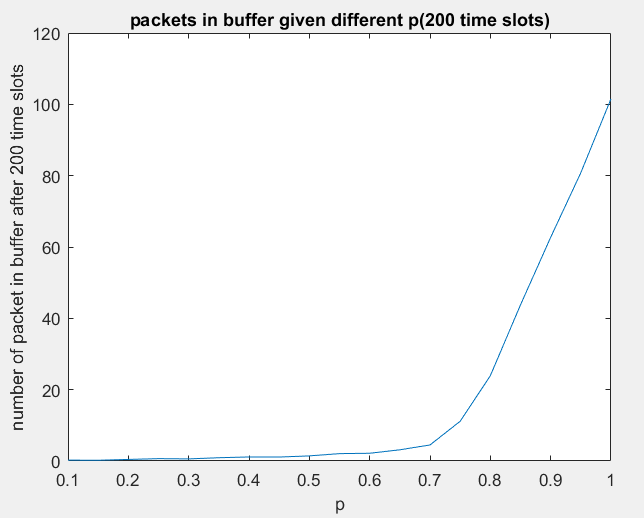
\includegraphics[width = 0.5\textwidth]{./data/numPacket-p.PNG}  
   \caption{number of packet in buffer after 200 time slot}
\end{figure}
Therefore, for r1 = r2 = 0.5, if we choose p less than 0.7 we may not have a HOL-blocking problem.
\begin{figure}[H]
   \centering
   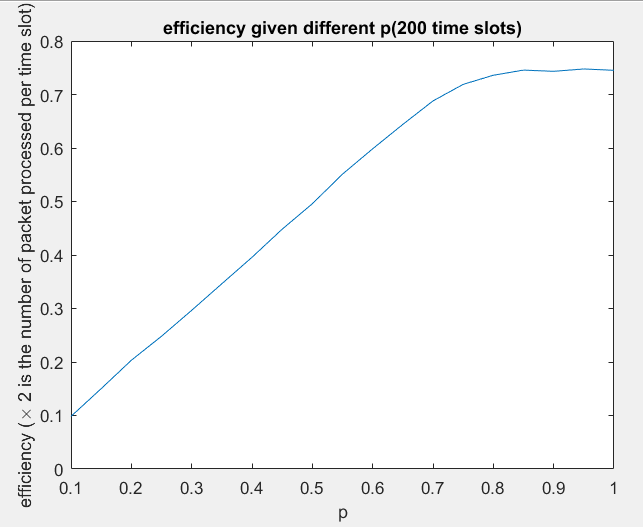
\includegraphics[width = 0.5\textwidth]{./data/efficiency.PNG}  
   \caption{efficiency given differnet p}
\end{figure}
Therefore, when p > 0.7, the efficiency seems to be steady to be around 0.75.\\
We can conclude that if we choose the p to be 0.7, the packet may not pile up in the buffer and still the switch has a good efficiency.\\
\noindent \textbf {To compute the 95\% confidence interval}\\
we choose p from 0.1 to 0.9,\\
\begin{tabular}{|| c | c ||}
 \hline \hline
 p & CI efficiency (\%) \\ \hline \hline
0.1 & [6.25,12.5]\\ \hline
0.2 & [15.50,23.25]\\ \hline
0.3 & [25.50,33.75]\\ \hline
0.4 & [35.50,45.50]\\ \hline
0.5 & [44.50,54.25]\\ \hline
0.6 & [54.25,64.25]\\ \hline
0.7 & [65.75,72.50]\\ \hline
0.8 & [70.0,77.0]\\ \hline
0.9 & [71.0,78.0]\\ \hline

\end{tabular}
\end{multicols*}
\newpage
\begin{multicols*}{2}
We just change the parameter $r_1,r_2$ in the function above and we can get the switch's behaviour when $r_1 = 0.75 ~and~ r_2 = 0.25$,query script:\\
\begin{lstlisting}
buffer = zeros(1,100);
k = 1;
for p = 0.1 : 0.05 : 1
    for i = 1 : 100
        [nstate,efficiency_lyc, efficiency_tu] = numberInInput(p,0.75,0.25,200);
        buffer(i) = sum(nstate);
        efficiency(i) = efficiency_tu;
    end
    recordNumber(k) = mean(buffer);
    recordEfficiency(k) = mean(efficiency);
    k = k+1;
end
plot(0.1:0.05:1,recordNumber);
title('packets in buffer given different p(200 time slots)');
xlabel('p');
ylabel('number of packet in buffer after 200 time slots');

plot(0.1:0.05:1,recordEfficiency);
title('efficiency given different p(200 time slots)');
xlabel('p');
ylabel('efficiency (\times 2 is the number of packet processed per time slot)');

\end{lstlisting}
\begin{figure}[H]
   \centering
   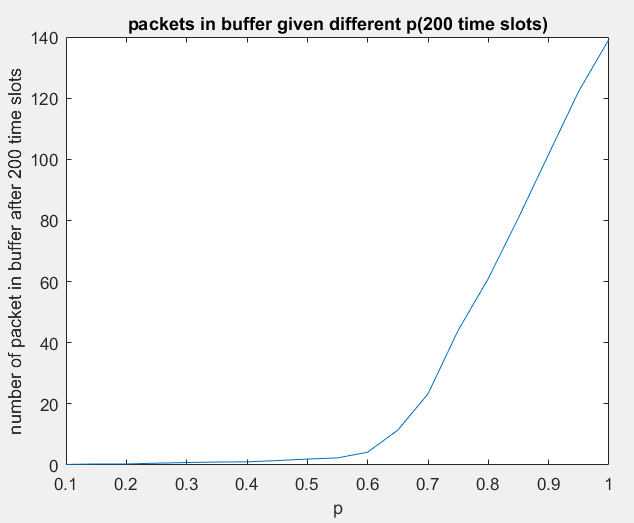
\includegraphics[width = 0.5\textwidth]{./data/numPacket-p2.png}  
   \caption{number of packet in buffer after 200 time slot}
\end{figure}
\begin{figure}[H]
   \centering
   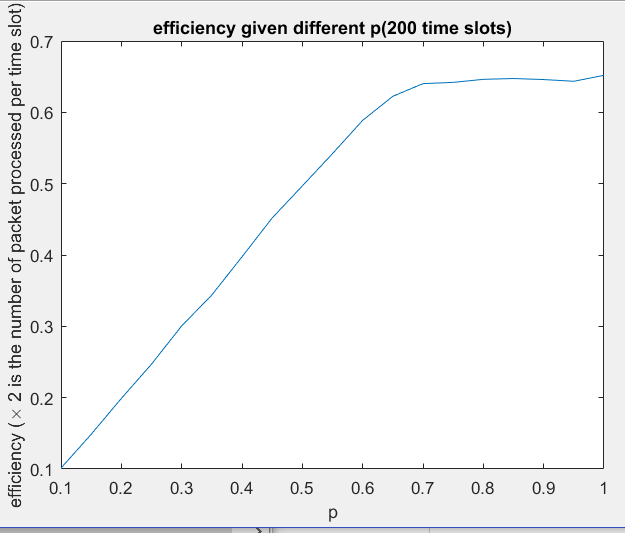
\includegraphics[width = 0.5\textwidth]{./data/efficiency2.png}  
   \caption{efficiency given differnet p}
\end{figure}
\begin{tabular}{|| c | c ||}
 \hline \hline
 p & CI efficiency (\%) \\ \hline \hline
0.1 & [7.75,12.75]\\ \hline
0.2 & [16.75,23.75]\\ \hline
0.3 & [25.50,34.50]\\ \hline
0.4 & [35.25,45.25]\\ \hline
0.5 & [43.75,53.75]\\ \hline
0.6 & [55.25,62.75]\\ \hline
0.7 & [60.75,67.00]\\ \hline
0.8 & [61.25,65.50]\\ \hline
0.9 & [60.75,70.55]\\ \hline 
\end{tabular}
\\Clearly, the efficiency decreases and it is more easily for the buffer to pile up packets.\\

\end{multicols*}





\section{Markov chain}
\subsection{\normalsize{Problem Description}}
We use Markov chain to simulate the Wright-Fisher model. The Wright-Fisher model produces successive generations with a 2-step process. The model first creates N pairs of parents selected randomly and with replacement from the population. Then each pair produces a single offspring with its genotype inherited by selecting one gene from each parent. All parents die after mating. The allele distribution x(t) is a Markov chain that advances by random sampling woth replacement from the pool of parent genes. The density of alleles evolves according to a binomial probability density. For example if we have two parents with A1A2,A1A2. So in the pool we have two A1 and two A2, the next time in the pool after mating, the probability we have 4 A2 next time is ${4 \choose 4}(\frac{2}{4})^4(1- (\frac{2}{4}))^0$, to generalize, if we have N parents in the pool and i is the number of A2 in the current state. the probability next state has j A2 conforms the following probability. \\
$P_{i,j} = {2N \choose j}(\frac{i}{2N})^j(1-\frac{i}{2N})^{2N-j}$

\subsection{\normalsize{Impletation}}
Using the previous knowledge, we can easily construct a transition matrix,we just need to give an initial state, and apply the transition matrix at every time slot. For example, if we have 1 parent, then, the i can be 0 1 2, j can be 0,1,2 ; the transition matrix is 
\[
\begin{matrix}
 & i=0 & i =1 & i = 2\\
 j = 0 & 1 & 0  & 0 \\
 j = 1 & \frac{1}{4} & \frac{1}{2} & \frac{1}{4} \\
 j = 2 & 0& 0 & 1
\end{matrix}
\]
if the parent is A1A2, then the initial input is [0,1,0] , and the output is $[\frac{1}{4},\frac{1}{2},\frac{1}{4}]$. That means the next time, there is probability of $\frac{1}{4}$ to have no A2 next time and so on. which is just $input * P$, therefore, just continue such Markov chain we may finally achieve a stable state.\\
\noindent \textbf {filename: genotypicSimulation.m}
\begin{lstlisting}
function [output,steadyState] = genotypicSimulation(N,evalBudget,input)
% output = genotypicSimulation(N,evalBudget,input)
%output is the output history of the experiment
%transition matrix 
if length(input) ~= 2 * N + 1
    disp('please input the right parameter');
end
P=zeros(2*N+1,2*N+1); 
 for i = 1:2*N+1
     for j = 1:2*N+1
         P(i,j) = nchoosek(2*N,j-1)*((i-1)/(2*N))^(j-1)*(1-(i-1)/(2*N))^(2*N-j+1);
     end 
 end
 
 output = zeros(evalBudget + 1,2 * N + 1); % record all output the first output is the input
 output(1,:) = input;
 for i = 1 : evalBudget
    output(i+1,:) = output(i,:) * P ;
    %a tolerance check to  automatically stop the simulation when the density is close to its steady-state
    LIT = ismembertol(output(i+1,:),output(i,:));
    if all(LIT == 1)  
        steadyState = output(i+1,:);
        break;
    end
end
\end{lstlisting}
\subsection{\normalsize{Result \& Analysis:}}
For the first situation, when all the parents have A1A2, we run the following script to get the result:
\begin{lstlisting}
clear
N = 100;
input = [zeros(1,N),1,zeros(1,N)];
[output,steadyState] = genotypicSimulation(N,10000,input);
\end{lstlisting}
\noindent \textbf {Note: for efficiency, when I was doing the experiment the transition matrix is generated only once and is not cleared in the work space so in every trial we do not need to generate it again};\\
\noindent \textbf {result:}\\
\noindent \textbf {[0.5,0,0,0,...,0,0,0.5]]}\\
So we have 0.5 chance to get all A1 and 0.5 chance to get all A2.\\
\noindent \textbf {change the input}
new script: we set i=98 in the initial state.
\begin{lstlisting}
N = 100;
input = [zeros(1,N-2),1,zeros(1,N+2)];
[output,steadyState] = genotypicSimulation(N,10000,input);
\end{lstlisting}
\noindent \textbf {result:}\\
\noindent \textbf {[0.51,0,0,0,...,0,0,0.49]]}\\
So we have 0.51 chance to get all A1, and 0.49 chance to get all A2.\\
\noindent \textbf {change the input}
new script: we set i=98 in the initial state.
\begin{lstlisting}
N = 100;
input = [zeros(1,N-49),1,zeros(1,N+49)];
[output,steadyState] = genotypicSimulation(N,10000,input);
\end{lstlisting}
\noindent \textbf {result:}\\
\noindent \textbf {[0.7450,0,0,0,...,0,0,0.2550]]}\\
So we have 0.7450 chance to get all A1, and 0.2550 chance to get all A2.\\
\noindent \textbf {Comments on the outcome}\\
That is, after a very long period of time, it is very rare for a generation in whose gene pool, both A1 and A2 exist. The gene pool would be either all A1 or all A2. If the initial situation has more A1 than A2, there will be larger probability to have all A1 after infinite generations.\\
\noindent \textbf {Why does this scenario seem to defy the assertion of the Perron-Frobenius theorem?}\\
The Perron-Frobenius theorem, proved by Oskar Perron(1907) and Georg Frobenius(1912), asserts that a real square matrix with positive entries has a unique largest real eigenvalue and that the corresponding eigenvector can be chosen to have strictly positive components, and also asserts a similar statement for certain classes of nonnegative matrices.\\
If we run the script `[V,D]= eig(A)', if N is 100, we got 201 eigenvalues and each corresponding to a eigenvector with all zeros. This seems to defy the Perron-Frobenius Theorm, but actually it did not becasue we know P is not a positive matrix. There are always 0's in the matrix.\\
\noindent \textbf {Why does this scenario seem to defy the Markov chain ergodic theorem}\\
Clearly, from the previous experiment, if we give different initial state, the Markov chain did not goes to the same steady state. This theorem is actually not suitable for this problem because the initial state we gave does not conform stationary distribution. Therefore, if we choose one initial state, the other initial state may not be `travelled' or to say we can not `ergodic' all the possible outcome in the sample space.For instance if we have an initial state [0,0,..,1,0,0,...0], then upon next state, all values in the vector become none zero and we can not go to another initial state again.\\ 
Therefore this scenario seem to defy the assertions of the Perron-Frobenius theorem and the Markov chain ergodic theorem.\\ 



\end{document}